\chapter{Solution}
In this chapter I will describe the implementation of CloudASR,
  I will stress key design choices...

\section{Architecture}
The key requirement for the architecture of CloudASR is scalability.


Thus, the platform had to be designed from the very beginning to be able to run on many machines.


\IDEA{pre fork model, it is not possible to fork on demand}
\IDEA{not blocking architecture}

The architecture as described in Figure~\ref{fig:architecture} consists of several types of nodes,
  namely \textbf{API}, \textbf{Web}, \textbf{Master}, \textbf{Worker} and \textbf{Recordings Saver}.
These nodes communicate with each other by sending messages over ZeroMQ sockets,
  which allows each node to run on different machine.
\TODO{cite: Viewing control structures as patterns of passing messages}

\begin{figure}
  \centering
  \includegraphics[width=0.75\textwidth]{./img/architecture.pdf}

  \label{fig:architecture}
  \caption{\TODO{Architecture}}
\end{figure}

\IDEA{Master-Slave architecture, multiple workers}
\TODOIMG{fig:queue}{Queue architecture}

Each node was implemented with two main design patterns in mind, namely Dependency Injection and Factory Method.
Usage of these patterns together with message oriented architecture made possible to test the whole platform easily,
  because it enabled to pass test doubles into the nodes
  and then send fake messages needed to test a correct behaviour.
As a result, a typical unit test structure looks like a test in Figure~\ref{fig:unit-test}.
\TODO{cite: Inversion of control containers and the dependency injection pattern}
\TODO{cite: Design patterns: Abstraction and reuse of object-oriented design}

In addition to unit tests there are also integration tests,
  which test the factory methods that create production ready nodes,
  and end-to-end tests,
  which test that both batch and online recognition mode requests are handled correctly.
This test suite ensures that developers did not break anything
  and it also gives them confidence to change the code without fear.

\begin{figure}
  \verbatiminput{snippets/unit_test.py}

  \label{fig:unit-test}
  \caption{An example of unit test structure.}
  \TODO{add better caption}
\end{figure}


\subsection{API}
The main task of the API container is to forward requests from the clients to the workers.
The requests are either in form of HTTP POST for the batch mode or Socket.IO for the online mode.
The API is built on top of Flask framework with enabled asynchronous processing
  which allows single API container to process many parallel requests,
  because there are no blocking operations in the API container -
  it just receives requests from clients and forwards them via ZeroMQ to the workers.

\subsection{Web}
\IDEA{Mention Annotation Interface and Webdemo also link to screenshots}
\IDEA{Describe process of annotation}
CloudASR platform also has a web interface.
The web interface distinguishes between two types of user roles: administrators and users.
Administrators can browse all recordings with their transcriptions and manage workers descriptions.
Normal users are only allowed to add transcriptions to the recordings.

\TODOIMG{fig:annotation-interface}{Screen of the Annotation Interface}


Finally, the Web hosts a demo (See Figure~\ref{fig:webdemo}) of the CloudASR platform,
  through which users can try out different workers directly in their web browsers.
The demo has two modes, namely, dictation mode that only shows the best transcription of the recording
  and evaluation mode that also allows users to confirm that the recording is correct.

\TODOIMG{fig:webdemo}{Screen of a Web Demo}

\subsection{Master}
\IDEA{queue for every language}
The main task of the Master is to keep track about running workers and scheduling tasks to them.
The Master keeps track about running workers which send heartbeats with information about their state
  and when the Api asks for a worker address the master can return address of an available worker.

The workers can be in four different states:
  \textbf{started}, \textbf{waiting}, \textbf{working} and \textbf{not responding}.
  and it sends four different heartbeats:
  \textbf{started}, \textbf{waiting}, \textbf{working} and \textbf{finished}.
The worker starts in in the \textbf{started} state,
  after that it moves to the \textbf{waiting} state by sending the \textbf{waiting} heartbeat.
The worker remains in the waiting state until \textbf{the Master assings a tasks} to it,
  then it moves to the \textbf{working} state
  where it remains as long as it is working.
In the working state worker sends working heartbeats periodically,
  to inform the Master that it is working and it did not fail.
At the end of the task the Worker sends \textbf{finished} heartbeat
  and the Master changes the state of the Worker to the \textbf{working} state.

Additionally, when a worker crashes during the processing of the task and it gets restarted,
  it sends started heartbeat again,
  which informs the Master, that the worker was restarted and it adds it to the queue again.

When a worker does not send any heartbeat for 10 seconds,
  the master set the worker state to \textbf{not responding}.
But as soon as the worker sends any heartbeat,
  the master will set the worker to the appropriate state.

This whole process can be seen as a finite automaton illustrated in Figure~\ref{fig:worker-state}.

\begin{figure}
  \centering
  \includegraphics[width=0.75\textwidth]{./img/worker-state.pdf}

  \label{fig:worker-state}
  \caption{\TODO{Worker state transition diagram}}
\end{figure}

Unfortunately, the Master is a single point of failure of CloudASR platform.
When the Master stops working no speech recognition requests can be processed,
  because the API containers will not know to which worker they can forward the request.
But as soon as the Master starts working the platform should be available again.


\subsection{Worker}




\IDEA{VAD}
\IDEA{Kaldi}
\IDEA{Heartbeats}
\blindtext

\subsection{Deployment of New Kaldi Worker}
\blindtext

\subsection{Deployment of Arbitrary Worker}
\blindtext

\subsection{Recordings saver}
The main task of the Recordings saver is to save and serve recordings processed by workers.
When the worker finishes recognition it sends the recording with its n-best hypotheses to the Recording saver via ZeroMQ socket.
The saver saves the wave file to the filesystem and it save the n-best hypotheses to the database so that they can be used in the future.

\TODOIMG{fig:db-schema}{Database schema}



\section{Request Workflow}
\blindtext

\subsection{Batch Recognition}
\blindtext

\TODOIMG{fig:batch}{Batch Workflow}

\subsection{Online Recognition}
\blindtext

\TODOIMG{fig:online}{Online Workflow}



\section{Deployment}
\blindtext

\subsection{Single-Host Deployment}
Single-Host deployment allows users to run CloudASR directly on their machines.
The only dependency for running CloudASR is Docker.
After that it is possible to use prepared Makefile to run CloudASR by command \texttt{make run\_locally}.
The platform can stopped by command \texttt{make stop}.

The Makefile is prepared to run only one worker with English TownInfo model.
In order to run different worker users have to edit the Makefile, especially the name of the worker Docker image.

\TODO{don't use Makefile, use some python script with same interface for Multi-Host Deployment}

\subsection{Multi-Host Deployment}
\blindtext
\TODO{describe Mesos installation}
\TODO{insert example cloudasr.json configuration for the deployment}

\subsection{Scalability}
\blindtext

\subsection{Contiunous Integration \& Countinuous Delivery}
\blindtext


\section{Discussion}
\IDEA{Compare throughput of Queue vs Master-Slave, discuss options}
\IDEA{different architectures solving Harddisk bottleneck, Network bottleneck}
